%&fmt.out/fmt

\begin{document}
%    \includeonlyframes{current}

    \title{Автоматическое обнаружение гонок при параллельных сборках на основе Make}
    \subtitle{Метод и реализация}
    \date{X июня 2024 г.}
    \author{Артем Климов, Владислав Иванишин, Александр Монаков}
    \institute{\!
\includegraphics[width=10em]{logo_RU_basic.png}}

    \captionsetup{font=footnotesize,labelformat=empty}

%% /usr/share/texlive/texmf-dist/tex/latex/beamertheme-metropolis/beamerinnerthememetropolis.sty
    \setbeamertemplate{title page}{
        \begin{minipage}[b][\paperheight]{\textwidth}
            \vspace*{1mm}
            \vfill%
            \ifx\inserttitle\@empty\else\usebeamertemplate*{title}\fi
            \ifx\insertsubtitle\@empty\else\usebeamertemplate*{subtitle}\fi
%%     \usebeamertemplate*{title separator}
            \ifx\beamer@shortauthor\@empty\else\usebeamertemplate*{author}\fi
            \ifx\insertdate\@empty\else\usebeamertemplate*{date}\fi
            \ifx\insertinstitute\@empty\else\usebeamertemplate*{institute}\fi
            \ifx\inserttitlegraphic\@empty\else\usebeamertemplate*{title graphic}\fi
            \vfill
            \vspace*{2mm}
        \end{minipage}
    }

    \begin{frame}[plain] % Don't show slide number on the title slide.
        \titlepage
        \note{
            Добрый день. Меня зовут Артем, я представляю работу "Автоматическое обнаружение гонок в параллельных
            сборках на основе Make".
        }
    \end{frame}

    \begin{frame}{План презентации}
        \begin{itemize}
            \setlength\itemsep{1.1em}
            \item \textbf{Введение}. Состояния гонок в Makefile. Примеры и формулировка проблемы.
            \item \textbf{Обзор существующих решений}.
            \item \textbf{Теоретический метод} автоматического обнаружения состояний гонок.
            \item \textbf{Реализация} метода в виде сантизатора для Make.
            \item \textbf{Оценка} сантизатора на реальных проектах, \textbf{сравнение} с существующими решениями. \textbf{Заключение}.
        \end{itemize}

        \note{
            В рамках этой работы мы исследуем проблему состояний гонок в схемах сборки и подробно
            рассмотрим новый разработанный нами инструмент, с помощью которого их можно значительно
            легче обнаруживать.
        }
    \end{frame}


    \section{Введение}

    \begin{frame}{Введение: Состояния гонок}

        \textbf{Состояние гонки} --- ситуация, когда несколько потоков работают с одним и тем же ресурсом одновременно,
        и результат выполнения программы зависит от порядка выполнения потоков.

        \begin{itemize}
            \item Одновременное чтение и запись по одному и тому же адресу;
            \item Создание каталога и одновременная работа с его содержимым;
            \item Удаление ресурса без ожидания окончания его использования.
        \end{itemize}

        \note{
            Итак, напомним, что такое состояние гонки в целом. Это ситуация, когда несколько потоков одновременно работают с \textbf{одним}
            ресурсом, и результат выполнения программы зависит от \textbf{порядка}, в котором они выполняются.
        }

    \end{frame}

    \begin{frame}{Введение: Состояния гонок}

        Пример: Два потока пытаются увеличить переменную \texttt{counter}, если она меньше 1.

        \lstinputlisting[language=C++]{src/racesample.cpp}

        С неудачным планированием переменная может быть увеличена дважды, и окончательное значение будет равно 2.

        \note{
            Обычно о состояниях гонок говорят в контексте языков программирования, таких как C++ или Java. В них гонки могут возникать из-за отсутствия синхронизации между процессами. Например, забытым мьютексом, как в примере на экране.
        }

    \end{frame}

    \begin{frame}{Введение: Состояния гонки в схемах сборки}
        \begin{itemize}
            \item Цели сборки могут собираться параллельно;
            \item При отсутствии необходимой синхронизации могут возникать гонки.
        \end{itemize}

        \begin{center}
            \begin{tikzpicture}
                \node[style=draw, minimum width=1.5cm] (libcpp) at (2,1.5) {lib.cpp};
                \node[style=draw, minimum width=1.5cm] (libo) at (4,1.5) {lib.o};
                \node[style=draw, minimum width=1.5cm] (liba) at (6,1.5) {lib.a};

                \node[style=draw, minimum width=3cm] (appcpp) at (2.75,0) {app.cpp};
                \node[style=draw, minimum width=3cm] (appo) at (6.25,0) {app.o};
                \node[style=draw, minimum width=3cm] (app) at (9.75,0) {app};

                \node[text width=5cm] at (10.5,1.1) {
                    \texttt{app} зависит от \texttt{lib.a}, но \textbf{не дожидается его сборки}
                };

                % liba -> app
                \draw[gray, dashed, line width=1pt, shorten >=2pt, shorten <=2pt, ->]
                (liba) to[out=0, in=180] ($(app.west) + (0, 0.12)$);

                % Common
                \node[minimum width=16cm, minimum height=3.5cm] (sizer) at (6.5,0.3) {};
                \node at (0,1.5) {Поток 1:};
                \node at (0,0) {Поток 2:};

                % appo -> app
                \draw[line width=1pt, shorten >=2pt, shorten <=2pt, ->]
                ($(appo.east) + (0,-0.12)$) -- ($(app.west) + (0,-0.12)$);

                % Time text and arrow
                \node[gray, font=\itshape] (time) at (11.4, -1.16) {$\tau$};
                \draw[gray, line width=0.7pt, ->] (0, -1.16) to (11, -1.16);

                \draw[line width=1pt, shorten >=2pt, shorten <=2pt, ->] (libcpp) -- (libo);
                \draw[line width=1pt, shorten >=2pt, shorten <=2pt, ->] (libo) -- (liba);
                \draw[line width=1pt, shorten >=2pt, shorten <=2pt, ->] (appcpp) -- (appo);
            \end{tikzpicture}
        \end{center}

        \note{
            Однако состояния гонок могут возникать и при сборке проектов. Там, вместо мьютексов, семафоров или условных переменных примитивами синхронизации являются зависимости между целями сборки. Отсутствие нужной зависимости, по аналогии с отсутствием мьютекса в предыдущем слайде, может привести к состоянию гонки.

            На слайде изображен процесс сборки некоторого проекта. В нём приложение может собираться параллельно с библиотекой, которую оно использует.

            Однако в схеме сборки не указано, что для компоновки приложения необходимо дождаться сборки библиотеки.
        }
    \end{frame}

    \begin{frame}{Введение: Состояния гонки в схемах сборки}
        \begin{itemize}
            \item Если сборка библиотеки затянется, произойдет ошибка:
        \end{itemize}

        \begin{center}
            \begin{tikzpicture}
                \node[style=draw, minimum width=2.2cm] (libcpp) at (2.35,1.5) {lib.cpp};
                \node[style=draw, minimum width=2.2cm] (libo) at (5.2,1.5) {lib.o};
                \node[style=draw, minimum width=2.2cm] (liba) at (8.05,1.5) {lib.a};

                \node[style=draw, minimum width=2cm] (appcpp) at (2.25,0) {app.cpp};
                \node[style=draw, minimum width=2cm] (appo) at (4.75,0) {app.o};
                \node[style=draw, minimum width=2cm] (app) at (7.25,0) {app};
                \node[red, style=draw, minimum width=2cm] (ошибка) at (9.75,0) {ошибка};

                \node[red, style=draw, dashed, minimum width=4cm] (error) at (3.5,0.75) {lib.a еще не готова};

                \draw[red, dashed, line width=1pt, shorten >=2pt, shorten <=2pt, ->]
                (error) to[out=0, in=180] ($(app.west) + (0, 0.12)$);

                \draw[red, line width=1pt, shorten >=2pt, shorten <=2pt, ->] (app) -- (ошибка);

                % Common
                \node[minimum width=16cm, minimum height=3.5cm] (sizer) at (6.5,0.3) {};
                \node at (0,1.5) {Поток 1:};
                \node at (0,0) {Поток 2:};

                % appo -> app
                \draw[line width=1pt, shorten >=2pt, shorten <=2pt, ->]
                ($(appo.east) + (0,-0.12)$) -- ($(app.west) + (0,-0.12)$);

                % Time text and arrow
                \node[gray, font=\itshape] (time) at (11.4, -1.16) {$\tau$};
                \draw[gray, line width=0.7pt, ->] (0, -1.16) to (11, -1.16);

                \draw[line width=1pt, shorten >=2pt, shorten <=2pt, ->] (libcpp) -- (libo);
                \draw[line width=1pt, shorten >=2pt, shorten <=2pt, ->] (libo) -- (liba);
                \draw[line width=1pt, shorten >=2pt, shorten <=2pt, ->] (appcpp) -- (appo);
            \end{tikzpicture}
        \end{center}

        \note{
            Если разработчику не повезёт и сборка библиотеки займёт много времени, то сборка всего проекта может завершиться неудачей.
        }
    \end{frame}

    \begin{frame}{Введение: Состояния гонки в схемах сборки}
        \begin{itemize}
            \item \textbf{Решение:} Определить пропущенную зависимость и добавить ее в схему сборки.
        \end{itemize}

        \begin{center}
            \begin{tikzpicture}
                \node[style=draw, minimum width=2.2cm] (libcpp) at (2.35,1.5) {lib.cpp};
                \node[style=draw, minimum width=2.2cm] (libo) at (5.2,1.5) {lib.o};
                \node[style=draw, minimum width=2.2cm] (liba) at (8.05,1.5) {lib.a};

                \node[style=draw, minimum width=2cm] (appcpp) at (2.25,0) {app.cpp};
                \node[style=draw, minimum width=2cm] (appo) at (4.75,0) {app.o};
                \node[style=draw, minimum width=2cm] (app) at (10.8,0) {app};

                \node[text width=3.6cm] at (8,0.5) {
                    \small{Поток 2 ждёт \texttt{lib.a} перед сборкой \texttt{app}}
                };

                % liba -> app
                \draw[line width=1pt, shorten >=2pt, shorten <=2pt, ->]
                (liba) to[out=0, in=180] ($(app.west) + (0, 0.12)$);

                % Common
                \node[minimum width=16cm, minimum height=3.5cm] (sizer) at (6.5,0.3) {};
                \node at (0,1.5) {Поток 1:};
                \node at (0,0) {Поток 2:};

                % appo -> app
                \draw[line width=1pt, shorten >=2pt, shorten <=2pt, ->]
                ($(appo.east) + (0,-0.12)$) -- ($(app.west) + (0,-0.12)$);

                % Time text and arrow
                \node[gray, font=\itshape] (time) at (11.4, -1.16) {$\tau$};
                \draw[gray, line width=0.7pt, ->] (0, -1.16) to (11, -1.16);

                \draw[line width=1pt, shorten >=2pt, shorten <=2pt, ->] (libcpp) -- (libo);
                \draw[line width=1pt, shorten >=2pt, shorten <=2pt, ->] (libo) -- (liba);
                \draw[line width=1pt, shorten >=2pt, shorten <=2pt, ->] (appcpp) -- (appo);
            \end{tikzpicture}
        \end{center}

        \note{
            Встретив такую ошибку, разработчик может либо попробовать ещё раз, либо разобраться в причине и добавить недостающую зависимость в схему, что устранило бы проблему.
        }
    \end{frame}

    \begin{frame}{Введение: Состояния гонок в реальных проектах}
        \tikz[remember picture, overlay] \node[text width=\textwidth, minimum width=\textwidth] at ($(current page.center)-(0,-2.5)$) {
            Ошибки сборки, связанные с состояниями гонок, часто становятся предметом обсуждения на форумах:
        };

        \tikz[remember picture, overlay] \node[anchor=center] at ($(current page.center)-(0,-0.5)$) {
            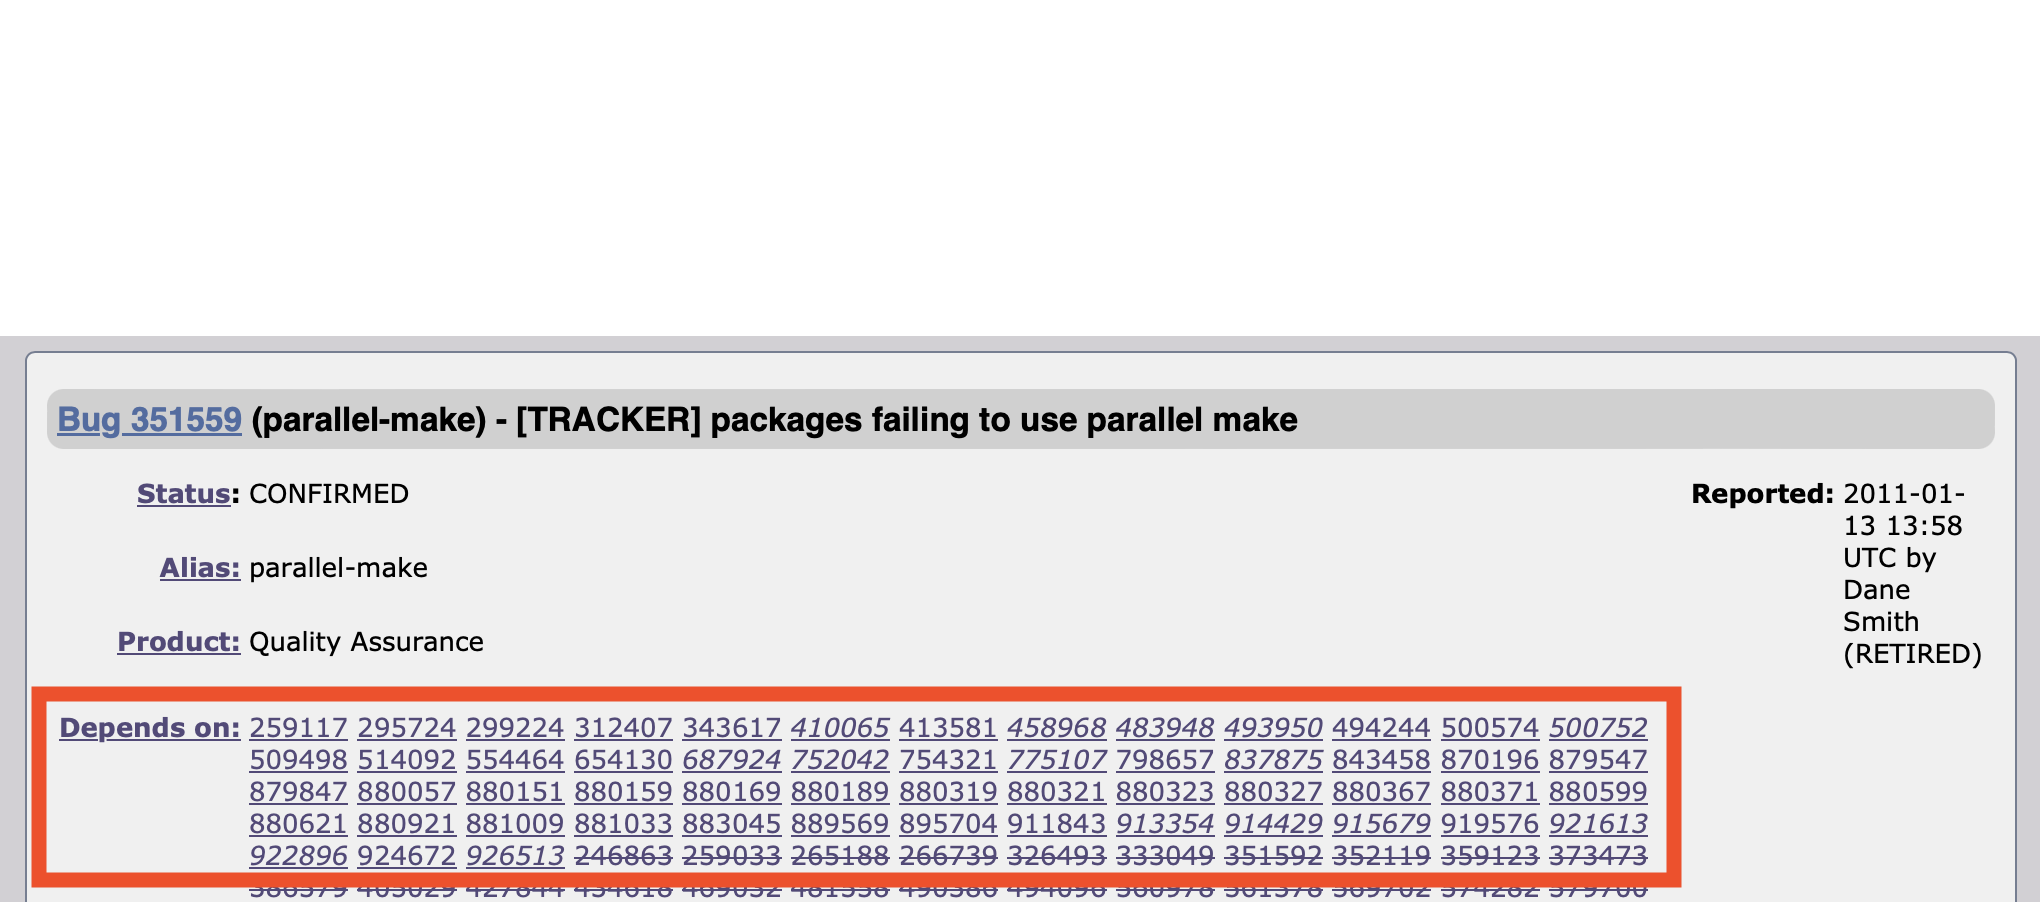
\includegraphics[width=1.1\textwidth]{gentoo-races}
        };

        \note{
            Состояния гонок часто проявляются как плавающие баги, которые трудно и редко воспроизводятся. В связи с этим, их сложно искать и отлаживать вручную. Подтверждение этому можно найти на форуме Gentoo, где в настоящее время открыто свыше 50 обсуждений на эту тему. Некоторые из них были открыты более 10 лет назад и по-прежнему остаются нерешенными.
        }
    \end{frame}

    \begin{frame}{Введение: Формулировка проблемы}

        Состояния гонок в схемах сборки являются актуальной проблемой:

        \begin{itemize}
            \item Сценарий гонки может редко воспроизводиться;
            \item Состояния гонок могут приводить не только к ошибкам сборки, но и к уязвимостям и проблемам в успешно собраннном проекте.
        \end{itemize}

        \textbf{Цель исследования:} Облегчить для разработчиков поиск и отладку состояний гонок в их схемах сборки путём разработки санитайзера. Требования к нему:

        \begin{itemize}
            \item Обнаруживать все гонки, связанные с отсутствующими зависимостями;
            \item Выдавать детерминированный результат;
            \item Легко встраиваться в проекты;
            \item Не требовать \texttt{-j1} или многократных пересборок.
        \end{itemize}

        \note{
            Состояния гонок коварны тем, что являются скрытой проблемой, которая может проявиться самым нежелательным образом. Спонтанная ошибка сборки --- даже не самое страшное ее проявление. Возможен сценарий, в котором состояния гонок могут привести к уязвимостям и другим проблемам в собранном проекте.

            Так мы приходим к \textbf{цели} нашего исследования: разработать инструмент, с помощью которого такие гонки можно будет искать автоматически, чтобы помочь разработчикам избежать таких проблем в своих проектах.

            Главная цель, которую преследует эта работа --- снизить время и усилия, требуемые для обнаружения и отладки состояния гонки. Инструмент должен быть прост в использовании, обнаруживать максимальное количество гонок в проекте за не более чем одну его пересборку.
        }
    \end{frame}


    \section{Обзор существующих решений}

    \begin{frame}{Обзор существующих решений: Bazel}
        \begin{itemize}
            \item Система сборки Bazel --- использует песочницы для устранения случайности.
            \item Каждая цель собирается в своей песоцнице.
            \item Каждая песочница имеет только файлы, собранные целями-зависимостями.
        \end{itemize}

        \begin{center}
            \begin{tikzpicture}
                \node[style=draw, rounded corners, inner xsep=7pt, inner ysep=7pt, align=center, minimum width=1.5cm, text width=1.5cm] (prereq1) at (0,0) {
                    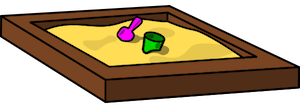
\includegraphics[width=1.5cm]{sandbox} \\
                    prereq1
                };
                \node[style=draw, rounded corners, inner xsep=7pt, inner ysep=7pt, align=center, minimum width=1.5cm, text width=1.5cm] (prereq2) at (0,-2) {
                    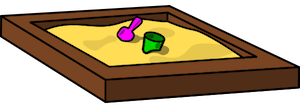
\includegraphics[width=1.5cm]{sandbox} \\
                    prereq2
                };
                \node[style=draw, rounded corners, inner xsep=7pt, inner ysep=7pt, align=center, minimum width=1.5cm, text width=1.5cm] (prereq3) at (10,0) {
                    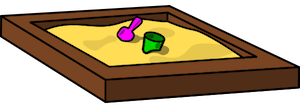
\includegraphics[width=1.5cm]{sandbox} \\
                    prereq3
                };
                \node[style=draw, rounded corners, inner xsep=7pt, inner ysep=7pt, align=center, minimum width=1.5cm, text width=1.5cm] (prereq4) at (10,-2) {
                    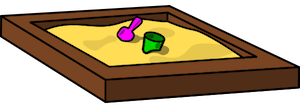
\includegraphics[width=1.5cm]{sandbox} \\
                    prereq4
                };

                \node[style=draw, rounded corners, inner xsep=7pt, inner ysep=7pt, align=center, minimum width=1.5cm, text width=1.5cm] (target) at (5,-1) {
                    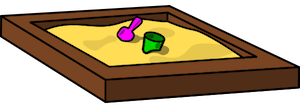
\includegraphics[width=1.5cm]{sandbox} \\
                    target
                };

                \draw[->, thick, shorten >=2pt, shorten <=2pt] (prereq1) to[out=0, in=180] (target);
                \draw[->, thick, shorten >=2pt, shorten <=2pt] (prereq2) to[out=0, in=180] (target);
                \draw[->, thick, shorten >=2pt, shorten <=2pt] (prereq3) to[out=180, in=0] (target);
                \draw[->, thick, shorten >=2pt, shorten <=2pt] (prereq4) to[out=180, in=0] (target);

                \node[rotate=-17] at (2.1, 0) {file1};
                \node[rotate=17] at (2.1, -2) {file2};
                \node[rotate=17] at (7.9, 0) {file3};
                \node[rotate=-17] at (7.9, -2) {file4};
            \end{tikzpicture}
        \end{center}

        \note{
            В современных системах сборки принимаются меры для борьбы с состояниями гонки. Например, Bazel позволяет производить сборку каждой цели в отдельной песочнице, в которой будут доступны только файлы, полученные в ходе сборки зависимостей. Это исключает гонки: с каждой такой виртуальной файловой системой работает одновременно лишь одна цель сборки, в определённом фиксированном порядке.
        }
    \end{frame}

    \begin{frame}{Обзор существующих решений: make {-}{-}shuffle}
        \begin{itemize}
            \item \texttt{make {-}{-}shuffle} --- перемешивает список пререквизитов каждой цели.
            \item Это увеличивает вероятность проявления гонки, но помогает не всегда.
        \end{itemize}

        \vspace{0.5cm}

        \begin{center}
            \texttt{target: prereq1, prereq2, prereq3, ...}

            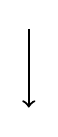
\begin{tikzpicture}
                \draw[->, thick] (0, 0) -- (0, -1);
            \end{tikzpicture}

            \texttt{target: prereq5, prereq2, prereq4, ...}
        \end{center}

        \note{
            Однако, Bazel и подобные системы пока не заменили собой классическую утилиту Make. Для неё существует только один известный мне инструмент, облегчающий поиск гонок. Это флаг \texttt{{-}{-}shuffle}, который позволяет случайным образом менять порядок сборки независимых целей, чтобы увеличить шанс проявления гонки. Однако, это требует полной пересборки проекта, может быть даже многократной. К тому же, как будет показано далее, многие гонки нельзя найти таким способом. Поэтому для дальнейшей работы выбрана именно система сборки Make.
        }
    \end{frame}


    \section{Теоретический метод}

    \newcommand{\raceframe}[2]{
        \begin{frame}
            \frametitle{Теоретический метод: #1}

            \conditionalText{#2}{1}{Самые частые состояния гонок, встречающиеся в реальных проектах, можно разделить на три категории:}

            \begin{itemize}
                \ifnum#2>2 \allgray \fi
                \ifnum#2=1 \allblack \fi
                \item \textbf{Гонка на содержимом файла.}
                \ifnum#2<3 \allgray \fi
                \ifnum#2=3 \allblack \fi
                \ifnum#2>3 \allgray \fi
                \ifnum#2=1 \allblack \fi
                \item \textbf{Гонка на пути к файлу.}
                \ifnum#2<4 \allgray \fi
                \ifnum#2=4 \allblack \fi
                \ifnum#2=1 \allblack \fi
                \item \textbf{Гонка между созданием каталога и файлом в нем.}
            \end{itemize}

            \vfill
        \end{frame}

        \ifnum #2=1
        \note{
            Самые \textbf{частые} состояния гонок, которые встречаются в \textbf{реальных} проектах, можно разделить на три категории. \textbf{Каждая} из них требует \textbf{свой подход} к обнаружению. Мы рассмотрим их\textbf{по очереди}.
        }
        \fi

        \ifnum #2=2
        \note{
            \textbf{Первая категория:} гонки на содержимом файлов.
        }
        \fi

        \ifnum #2=3
        \note{
            \textbf{Вторая категория:} гонки на путях к файлам.
        }
        \fi

        \ifnum #2=4
        \note{
            \textbf{Третья категория:} гонки между созданием каталога и его содержимым.
        }
        \fi
    }

    \raceframe{Типы гонок}{1}
    \raceframe{Гонка на содержимом файла}{2}

    \begin{frame}{Теоретический метод: Гонка на содержимом файла}

        В следующем Makefile присутствует гонка на содержимом файла \texttt{file.out}

        \begin{columns}[t]
            \begin{column}{.3 \textwidth}
                \newline
                \only<1,2>{
                    \lstinputlisting[
                        aboveskip=-\baselineskip,
                        basicstyle=\ttfamily,
                        language=bash,
                        escapechar=\%,
                        morekeywords={all, write_a, append_b}
                    ]{src/file-content-race-1.make}
                }
                \only<3>{
                    \lstinputlisting[
                        aboveskip=-\baselineskip,
                        basicstyle=\ttfamily,
                        language=bash,
                        escapechar=\%,
                        morekeywords={all, write_a, append_b}
                    ]{src/file-content-race-1-fixed.make}
                }
            \end{column}
            \begin{column}{.4 \textwidth}
                \newline \newline \newline
                \textit{\texttt{'a'} записывается в \texttt{file.out}}
                \newline
                \textit{из цели \texttt{write\_a}.}
                \newline
                \newline
                \textit{\texttt{'b'} добавляется к}
                \newline
                \textit{тому же файлу из цели}
                \newline
                \textit{\texttt{append\_b}.}
            \end{column}
        \end{columns}

        \vspace{1.2em}
        \visible<2->{
            \keyword{write\_a} и \keyword{append\_b} независимы, их порядок выполнения не определен.

            \texttt{file.out} может содержать \texttt{'ab'} или \texttt{'a'}.
        }

        \visible<3->{
            \textbf{Решение:} Добавить зависимость между \texttt{append\_b} и \texttt{write\_a}
        }

        \note{
            Рассмотрим этот тип гонки на примере.

            В этом мейкфайле цели \keyword{write\_a} и \keyword{append\_b} записывают какой-то текст в один и тот же файл. Однако они не зависят друг от друга, то есть \textbf{порядок} их \textbf{выполнения} не определён.

            В результате в файле \texttt{file.out} может оказаться либо \texttt{'ab'}, либо \texttt{'a'}.

            Чтобы исправить эту ситуацию, нужно сделать цель \texttt{append\_b} зависимой от \texttt{write\_a}.

            Итак, сейчас мы посмотрели на мейкфайл глазами, увидели проблему, и поняли, что надо сделать, чтобы её решить...
        }
    \end{frame}

    \begin{frame}{Теоретический метод: Гонка на содержимом файла}
        \begin{center}
            \textbf{\large{Как можно обнаружить такие состояния гонок?}}
        \end{center}

        \note{
            ...Но как можно обнаруживать такие гонки автоматически?
        }
    \end{frame}

    \begin{frame}{Теоретический метод: Гонка на содержимом файла}

        \textbf{Strace} --- утилита Linux, которая перехватывает и выводит системные вызовы и сигналы.

        \lstinputlisting[morekeywords={O_WRONLY}]{src/strace-log.txt}

        Согласно журналу strace, при сборке \texttt{file.out} открывается на запись двумя процессами.

        \note{
            Предлагается запустить сборку под strace. Strace - это утилита, которая перехватывает системные вызовы и сигналы, и печатает их в консоль.

            На самом деле strace не используется в готовом инструменте, но на таком примере будет проще понять, что на самом деле происходит.

            Итак, в логе strace для нашего примера видно, что файл \texttt{file.out} открывается двумя разными процессами.
        }
    \end{frame}

    \begin{frame}{Теоретический метод: Гонка на содержимом файла}
        Зная соответствие между процессами и породившими их целями, можно утверждать, что:

        \begin{enumerate}
            \item Цель \keyword{write\_a} производит запись в \texttt{file.out}
            \item Цель \keyword{append\_b} тоже производит запись в \texttt{file.out}
        \end{enumerate}

        \pause
        Граф зависимостей схемы сборки выглядит следующим образом:

        \begin{center}
            \begin{tikzpicture}[every node/.style = draw]
                \node[inner xsep=7pt] (append) at (0,0) {append\_b};
                \node[inner xsep=7pt] (write) at (0,1.2) {write\_a};
                \node[inner xsep=7pt] (all) at (3,0.6) {all};


                \only<3> \draw[line width=1pt, shorten >=2pt, shorten <=2pt, <->] (append) -- (write);
                \only<3> \draw[red, line width=1pt, -] (-0.2,0.5) -- (0.2,0.7);
                \only<3> \draw[red, line width=1pt, -] (0.2,0.5) -- (-0.2,0.7);

                \graph {
                    (write) ->[line width=1pt, shorten >=2pt, shorten <=2pt] (all);
                    (append) ->[line width=1pt, shorten >=2pt, shorten <=2pt] (all);
                };
            \end{tikzpicture}
        \end{center}
        \pause
        Так как между \texttt{write\_a} и \texttt{append\_b} нет ориентированного пути, цели являются независимыми и образуют гонку.

        \note {
            Если обработать этот лог и заменить процессы на имена целей, то можно получить более информативную последовательность событий, из которой можно зафиксировать, что цели \keyword{write\_a} и \keyword{append\_b} записывают что-то в один и тот же файл.

            Теперь обратимся к графу зависимостей. В нем видно, что цели \keyword{write\_a} и \keyword{append\_b} не зависят друг от друга --- между ними нет ориентированного пути. А поскольку прежде мы зафиксировали что они записывают что-то в один и тот же файл --- мы можем справедливо заявить о гонке.
        }
    \end{frame}

    \begin{frame}{Теоретический метод: Гонка на содержимом файла}
        \textbf{Обзор алгоритма:}
        \begin{enumerate}
            \item Запустить сборку под strace;
            \item Сопоставить процессы с целями; \only<2->{\textcolor{red}{--- Как?}}
            \item Получить граф зависимостей; \only<2->{\textcolor{red}{\strut --- Как?}}
            \item Найти недостающие зависимости между доступами к \\ одному и тому же \only<1,2>{\colorbox{white}{\strut пути}}\only<3>{\colorbox{diffrem}{\strut пути}}. \visible<3->{\textcolor{red}{--- Всегда ли путь $=$ файл?}}
        \end{enumerate}

        \note {
            Итак, давайте кратко подытожим вышесказанное. Чтобы автоматически находить гонки, нужно
            получить лог событий, граф зависимостей, а после для каждой пары конфликтующих доступов
            убедиться, что цели, которые их совершили, зависят друг от друга, то есть между ними есть
            ориентированный путь в графе зависимостей. Если его нет, то это гонка, и о ней можно сообщить.

            Однако, есть несколько проблем. Во-первых --- неясно, как сопоставить процессы с целями, которые они собирали.

            Во-вторых --- нам нужно как-то получить граф зависимостей, и это нетривиальная задача.

            Но эти две проблемы мы отложим на потом, а сейчас сосредоточимся на другом --- что делать с жёсткими ссылками?
        }
    \end{frame}

    \begin{frame}{Теоретический метод: Гонка на содержимом файла}
        \textbf{Жесткие ссылки} - это несколько имен для одного и того же файла в файловой системе. Они создаются с помощью команды \texttt{ln}.

        \begin{columns}[t]
            \begin{column}{.35 \textwidth}
                \newline
                \lstinputlisting[
                    aboveskip=-\baselineskip,
                    basicstyle=\ttfamily,
                    language=bash,
                    morekeywords={all}
                ]{src/file-content-race-2.make}
            \end{column}
            \begin{column}{.5 \textwidth}
                \newline \newline \newline \newline
                \textit{\texttt{hardlink\_a} и \texttt{hardlink\_b} - жесткие ссылки на \texttt{file.out}}
                \newline
                \newline
                \newline
                \textit{\texttt{'a'} записывается в \texttt{hardlink\_a} из цели}
                \newline
                \texttt{write\_a}
                \newline
                \newline
                \textit{\texttt{'b'} добавляется к \texttt{hardlink\_b} из цели}
                \newline
                \texttt{append\_b}
            \end{column}
        \end{columns}

        \note {
            Жёсткие ссылки позволяют давать одному и тому же файлу несколько путей в файловой системе. Они могут сбить с толку наш алгоритм, поскольку он полагается на то, что каждый файл уникально идентифицируется своим путём.

            В этом мейкфайле происходит то же самое, что и в предыдущем, но цели \keyword{write\_a} и \keyword{append\_b} работают с одним и тем же файлом не напрямую, а через две разные жесткие ссылки.
        }
    \end{frame}

    \begin{frame}{Теоретический метод: Гонка на содержимом файла}
        Журнал strace для предыдущей сборки укажет на следующее:

        \begin{itemize}
            \item Цель \keyword{file.out} производит запись в \texttt{file.out}
            \item Цель \keyword{write\_a} производит запись в \texttt{hardlink\_a}
            \item Цель \keyword{append\_b} производит запись в \texttt{hardlink\_b}
        \end{itemize}

        Все три пути различаются. Состояние гонки найти не удастся.

        \note{
            Из-за этого в журнале strace все доступы к этому файлу производятся через разные пути.
            Поэтому наш алгоритм не сможет обнаружить гонку - он будет думать, что все эти доступы относятся к трём разным файлам.
        }

    \end{frame}

    \begin{frame}{Теоретический метод: Гонка на содержимом файла}
        \textbf{Решение:} Использовать \textbf{номера inode} вместо путей к файлам.

        Номер inode --- уникальный идентификатор файла в файловой системе. У жестких ссылок на один и тот же файл номер inode совпадает. Для предыдущего примера:

        \begin{itemize}
            \item Цель \keyword{file.out} производит запись на inode \texttt{100000}
            \item Цель \keyword{write\_a} производит запись на inode \texttt{100000}
            \item Цель \keyword{append\_b} производит запись на \texttt{100000}
        \end{itemize}

        \note {
            Это можно исправить, если вместо путей к файлу использовать номера \texttt{inode}.

            Номер inode --- это уникальный идентификатор файла в файловой системе. Он гарантированно будет иметь одно и то же значение для всех жёстких ссылок на один и тот же файл.

            Если заменить пути к файлам на номера \texttt{inode}, то теперь \textbf{можно} увидеть, что эти три доступа на самом деле производятся к одному и тому же файлу.
        }
    \end{frame}

    \begin{frame}{Теоретический метод: Гонка на содержимом файла}
        \textbf{Обновленный алгоритм:}

        \begin{enumerate}
            \item Запустить сборку под трассировщиком с логированием inode;
            \item Сопоставить процессы с целями;
            \item Получить граф зависимостей;
            \item Найти недостающие зависимости между доступами к \\ одному и тому же \colorbox{diffrem}{\sout{\vphantom{fp}пути файла}}
            \colorbox{diffadd}{\vphantom{fp}номеру inode}
        \end{enumerate}

        Этот алгоритм может найти состояния гонок даже при использовании жестких ссылок.

        \note {
            И теперь, если соответствующим образом отредактировать сам алгоритм поиска, то он корректно
            найдет гонку из последнего примера.

            Однако при реализации алгоритма нужно быть внимательным, поскольку номера \texttt{inode} могут быть переиспользованы.
            Если игнорировать этот факт, то можно получить ложные срабатывания.
        }
    \end{frame}

    \raceframe{Гонка на пути к файлу}{3}

    \begin{frame}{Теоретический метод: Гонка на пути к файлу}

        В следующем Makefile присутствует гонка на пути \texttt{tmp\_file}

        \begin{columns}[t]
            \begin{column}{.45 \textwidth}
                \newline
                \lstinputlisting[
                    aboveskip=-\baselineskip,
                    basicstyle=\ttfamily,
                    language=bash,
                    morekeywords={all, something, something_else, rm}
                ]{src/file-path-race-3.make}
            \end{column}
            \begin{column}{.4 \textwidth}
                \newline \newline \newline \newline
                \texttt{tmp\_file} используется как временный файл.
                \newline
                Он удаляется после сборки цели.
                \newline \newline \newline
                То же имя используется для
                \newline
                временного файла в другой
                \newline
                цели.
            \end{column}
        \end{columns}

        Цели образуют гонку: \texttt{rm} может удалить файл, пока другая цель ещё использует его.

        \note {
            В этом примере присутствуют две независимые цели, использующие один и тот же временный файл \texttt{tmp\_file}.
            В каждой из них файл создается, используется, а потом удаляется.

            Это гонка, поскольку команда \texttt{rm} может быть выполнена, пока другая цель ещё использует файл.
        }
    \end{frame}

    \begin{frame}{Теоретический метод: Гонка на пути к файлу}
        Последовательность событий для примера выше:

        \begin{itemize}
            \item Цель \keyword{something} создаёт inode 10000
            \item Цель \keyword{something} удаляет inode 10000
            \item Цель \keyword{someting\_else} создаёт inode 10001
            \item Цель \keyword{something\_else} удаляет inode 10001
        \end{itemize}

        Номера inode не помогут обнаружить гонку на пути к файлу.

        \pause
        \textbf{Решение:} Использовать и пути, и номера inode для поиска гонок.

        \note {
            Рассмотрим лог событий для этого примера. Можно заметить, что после удаления и повторного создания наш
            временный файл получил другой номер \texttt{inode}. Поэтому алгоритм, основанный на номерах \texttt{inode},
            не сможет обнаружить эту гонку.

            С другой стороны, если бы мы всё еще использовали пути к файлам, то смогли бы обнаружить эту гонку, поскольку
            встретили бы конфликтующие доступы на удаление и запись из разных целей.

            Из этого можно сделать вывод, что в дополнение к номерам \texttt{inode} всё-таки нужно использовать пути к
            файлам. Но это нужно только для обнаружения гонок с участием удаления. По этой причине эти гонки и
            были вынесены во вторую категорию --- для них требуется немного другой алгоритм.
        }
    \end{frame}

    \raceframe{Гонка на каталоге}{4}

    \begin{frame}{Теоретический метод: Гонка на каталоге}

        Makefile ниже содержит гонку между созданием каталога и файлом в нем:

        \lstinputlisting[
            basicstyle=\ttfamily,
            language=bash,
            morekeywords={all, mkdir}
        ]{src/directory-race-4.make}

        Если доступ к директории (\keyword{echo}) выполнится раньше её создания (\keyword{mkdir}), произойдет ошибка.

        \note {
            Название категории говорит само за себя. Одна цель создаёт папку, а другая создаёт в ней какой-то файл.
            Однако, зависимость между этими целями не указана, и если они исполнятся в обратном порядке, то
            произойдет ошибка.

            Наш алгоритм пока не умеет находить такие гонки, поскольку папка и её содержимое --- это разные файлы,
            с разными путями и разными номерами inode.

            Чтобы исправить это, предлагается для каждого доступа к файлу добавлять в лог событий дополнительное событие
            \keyword{dir\_lookup} для родительской директории.

            Теперь последовательность событий будет выглядеть так, и в ней можно найти гонку между созданием папки и
            доступом к ней --- операцией \keyword{dir\_lookup}.
        }
    \end{frame}

    \begin{frame}{Теоретический метод: Гонка на каталоге}

        \textbf{Решение}: Сопровождать каждый доступ к файлу событием \keyword{dir\_lookup} для родительской директории:

        \vspace{0.5cm}

        \begin{tikzpicture}
            \node at (3.5,4) {Процессы:};
            \node at (12,4) {Файловая система:};

            \node[style=draw, minimum width=5cm, minimum height=0.9cm] (mkdir) at (3.5,3) {\texttt{\keyword{mkdir} build}};
            \node[style=draw, minimum width=5cm, minimum height=1.9cm] (echo) at (3.5,1.5) {\texttt{\keyword{echo} > build/a.out}};

            \node[align=left, text width=3cm] (build) at (12.5,3) {\texttt{./build}};
            \node[align=left, text width=3cm] (buildaout) at (12.5,1) {\texttt{./build/a.out}};

            \only<1> \draw[->, shorten >=4pt, shorten <=4pt] (6,3) -- (11,3);
            \only<1> \draw[-, shorten <=4pt] (6,2) -- (9,2);
            \only<1> \draw[->, shorten >=4pt] (9,2) to[in=180, out=0] (11,3);

            \only<2> \draw[red, thick, ->, shorten >=4pt, shorten <=4pt] (6,3) -- (11,3);
            \only<2> \draw[red, thick, -, shorten <=4pt] (6,2) -- (9,2);
            \only<2> \draw[red, thick, ->, shorten >=4pt] (9,2) to[in=180, out=0] (11,3);

            \draw[->, shorten >=4pt, shorten <=4pt] (6,1) -- (11,1);

            \only<1> {\node at (7.7, 3.3) {\texttt{write}}};
            \only<1> {\node at (7.7, 2.3) {\texttt{dir\_lookup}}};

            \only<2> {\node[red] at (7.7, 3.3) {\texttt{\textbf{write}}}};
            \only<2> {\node[red] at (7.7, 2.3) {\texttt{\textbf{dir\_lookup}}}};

            \node at (7.7, 1.3) {\texttt{write}};

            \node[gray, font=\itshape] (time) at (0.5, 0.5) {$\tau$};
            \draw[gray, line width=0.7pt, ->] (0.5, 4) to (0.5, 1);
        \end{tikzpicture}

        \visible<2> {
            Конфликт между \textcolor{red}{\texttt{write}} и \textcolor{red}{\texttt{dir\_lookup}} для \texttt{build} позволит найти гонку.
        }

        \note {

        }
    \end{frame}

    \begin{frame}{Теоретический метод: Гонка на каталоге}

        Такой подход работает с любой глубиной вложенности:

        \vspace{0.5cm}

        \begin{tikzpicture}
            \node at (3,6) {Процессы:};
            \node at (12,6) {Файловая система:};

            \node[style=draw, minimum width=5cm, minimum height=0.9cm] (mkdir) at (3.5,5) {\texttt{\keyword{mkdir} build}};
            \node[style=draw, minimum width=5cm, minimum height=1.9cm] (mkdir) at (3.5,3.5) {\texttt{\keyword{mkdir} build/foo}};
            \node[style=draw, minimum width=5cm, minimum height=1.9cm] (echo) at (3.5,1.5) {\texttt{\keyword{echo} > build/foo/a.out}};

            \node[align=left, text width=3cm] (build) at (12.5,5) {\texttt{./build}};
            \node[align=left, text width=3cm] (buildfoo) at (12.5,3) {\texttt{./build/foo}};
            \node[align=left, text width=3cm] (buildfooaout) at (12.5,1) {\texttt{./build/foo/a.out}};

            \draw[thick, red, ->, shorten >=4pt, shorten <=4pt] (6,3) -- (11,3);
            \draw[thick, red, -, shorten <=4pt] (6,2) -- (9,2);
            \draw[thick, red, ->, shorten >=4pt] (9,2) to[in=180, out=0] (11,3);

            \draw[->, shorten >=4pt, shorten <=4pt] (6,1) -- (11,1);

            \draw[thick, blue, ->, shorten >=4pt, shorten <=4pt] (6,5) -- (11,5);
            \draw[thick, blue, -, shorten <=4pt] (6,4) -- (9,4);
            \draw[thick, blue, ->, shorten >=4pt] (9,4) to[in=180, out=0] (11,5);

            \node[blue] at (7.7, 5.3) {\texttt{\textbf{write}}};
            \node[blue] at (7.7, 4.3) {\texttt{\textbf{dir\_lookup}}};
            \node[red] at (7.7, 3.3) {\texttt{\textbf{write}}};
            \node[red] at (7.7, 2.3) {\texttt{\textbf{dir\_lookup}}};
            \node at (7.7, 1.3) {\texttt{write}};

            \node[gray, font=\itshape] (time) at (0.5, 0.5) {$\tau$};
            \draw[gray, line width=0.7pt, ->] (0.5, 6) to (0.5, 1);
        \end{tikzpicture}

        \note {

        }
    \end{frame}

    \begin{frame}{Теоретический метод: Гонка на каталоге}

        \textbf{Проблема:} Каталоги могут создаваться по необходимости из разных мест:
        \lstinputlisting[
            basicstyle=\ttfamily,
            language=bash,
            morekeywords={all, lib1, lib9},
            escapechar=\%
        ]{src/directory-race-5.make}

        \note {
            Однако этого оказывается недостаточно. Дело в том, что в некоторых проектах директория сборки создаётся
            в каждой цели отдельно, несмотря на то грамотнее было бы выделить её создание в отдельную цель.

            В этом случае в логе событий будет несколько событий \keyword{write} для одной и той же директории.
            При этом только первое создание будет успешным, остальные просто не смогут повторно создать уже существующую
            папку.

            В результате алгоритм обнаружения гонок будет сообщать о ложных гонках между любыми двумя целями, которые
            обращаются к одной и той же директории сборки, хотя на самом деле это не гонка. Как избежать этих ложных
            срабатываний?
        }
    \end{frame}

    \begin{frame}{Теоретический метод: Гонка на каталоге}

        \begin{itemize}
            \item При множественных \keyword{mkdir} алгоритм выдаст ложные срабатывания.
        \end{itemize}

        \vspace{0.1cm}

        \begin{tikzpicture}
            \node[style=draw, minimum width=5cm, minimum height=0.9cm] at (3.5,3) {\texttt{\keyword{lib1}: \keyword{mkdir} build}};
            \node[style=draw, minimum width=5cm, minimum height=0.9cm] at (3.5,2) {\texttt{\keyword{lib2}: \keyword{mkdir} build}};
            \node[style=draw, minimum width=5cm, minimum height=1.9cm] at (3.5,0.5) {\texttt{\keyword{lib2}: \keyword{build\_library}}};

            \node[align=left, text width=3cm] (build) at (12.5,3) {\texttt{./build}};
            \node[align=left, text width=3cm] (buildaout) at (12.5,0) {\texttt{./build/lib1.a}};

            \draw[-, shorten <=4pt] (6,2) -- (9,2);
            \draw[-] (8.9,1.9) -- (9.1,2.1);
            \draw[-] (9.1,1.9) -- (8.9,2.1);

            \only<1> \draw[->, shorten >=4pt, shorten <=4pt] (6,3) -- (11,3);
            \only<1> \draw[-, shorten <=4pt] (6,1) -- (9,1);
            \only<1> \draw[->, shorten >=4pt] (9,1) to[in=180, out=0] (11,3);

            \only<2> \draw[red, thick, ->, shorten >=4pt, shorten <=4pt] (6,3) -- (11,3);
            \only<2> \draw[red, thick, -, shorten <=4pt] (6,1) -- (9,1);
            \only<2> \draw[red, thick, ->, shorten >=4pt] (9,1) to[in=180, out=0] (11,3);

            \draw[->, shorten >=4pt, shorten <=4pt] (6,0) -- (11,0);

            \only<1> \node at (7.7, 3.3) {\texttt{write}};
            \node at (7.7, 2.3) {failed \texttt{write}};
            \only<1> \node at (7.7, 1.3) {\texttt{dir\_lookup}};

            \only<2> \node[red] at (7.7, 3.3) {\texttt{\textbf{write}}};
            \only<2> \node[red] at (7.7, 1.3) {\texttt{\textbf{dir\_lookup}}};

            \node at (7.7, 0.3) {\texttt{write}};

            \node[gray, font=\itshape] (time) at (0.5, -1) {$\tau$};
            \draw[gray, line width=0.7pt, ->] (0.5, 3.5) to (0.5, -0.5);
        \end{tikzpicture}

        \visible<2>{
            \begin{itemize}
                \item Доступы из \keyword{lib1} и \keyword{lib2} будут считаться конфликтующими, хотя это не так.
            \end{itemize}
        }
    \end{frame}

    \begin{frame}{Теоретический метод: Гонка на каталоге}

        \begin{itemize}
            \item \textbf{Решение}: Для \keyword{dir\_lookup} искать любой зависимый предшествующий \keyword{write}, даже если он неуспешный.
        \end{itemize}

        \vspace{0.1cm}

        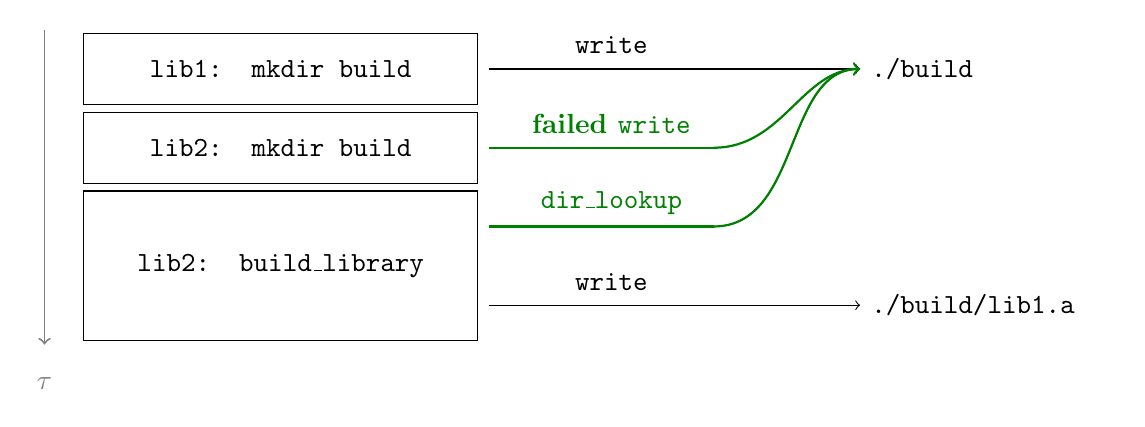
\begin{tikzpicture}
            \node[style=draw, minimum width=5cm, minimum height=0.9cm] at (3.5,3) {\texttt{\keyword{lib1}: \keyword{mkdir} build}};
            \node[style=draw, minimum width=5cm, minimum height=0.9cm] at (3.5,2) {\texttt{\keyword{lib2}: \keyword{mkdir} build}};
            \node[style=draw, minimum width=5cm, minimum height=1.9cm] at (3.5,0.5) {\texttt{\keyword{lib2}: \keyword{build\_library}}};

            \node[align=left, text width=3cm] (build) at (12.5,3) {\texttt{./build}};
            \node[align=left, text width=3cm] (buildaout) at (12.5,0) {\texttt{./build/lib1.a}};

            \draw[->, shorten >=4pt, shorten <=4pt] (6,3) -- (11,3);
            \draw[green!50!black, thick,  -, shorten <=4pt] (6,2) -- (9,2);
            \draw[green!50!black, thick,  ->, shorten >=4pt] (9,2) to[in=180, out=0] (11,3);

            \draw[-, shorten <=4pt] (6,1) -- (9,1);
            \draw[->, shorten >=4pt] (9,1) to[in=180, out=0] (11,3);

            \draw[green!50!black, thick, -, shorten <=4pt] (6,1) -- (9,1);
            \draw[green!50!black, thick, ->, shorten >=4pt] (9,1) to[in=180, out=0] (11,3);

            \draw[->, shorten >=4pt, shorten <=4pt] (6,0) -- (11,0);

            \node at (7.7, 3.3) {\texttt{write}};
            \node[green!50!black] at (7.7, 2.3) {\textbf{failed \texttt{write}}};
            \node[green!50!black] at (7.7, 1.3) {\textbf{\texttt{dir\_lookup}}};

            \node at (7.7, 0.3) {\texttt{write}};

            \node[gray, font=\itshape] (time) at (0.5, -1) {$\tau$};
            \draw[gray, line width=0.7pt, ->] (0.5, 3.5) to (0.5, -0.5);
        \end{tikzpicture}

        \begin{itemize}
            \item Оба выделенных доступа относятся к \keyword{lib2}, поэтому гонки нет.
        \end{itemize}
    \end{frame}


    \section{Реализация}

    \begin{frame}{Реализация: Архитектура}
        Сбор данных:
        \begin{itemize}
            \item \textbf{Граф зависимостей, соответствие процессов и целей} --- патч для Make.
            \item \textbf{Журнал событий} --- \texttt{ptrace}-трассировщик на Си вместо \texttt{strace}.
        \end{itemize}

        Архитектура:

        \begin{center}
            \begin{tikzpicture}
                \node[style=draw, rounded corners, inner xsep=10pt, inner ysep=6pt] (parmasan) at (-1, 0) {Санитайзер};
                \node[style=draw, rounded corners, inner xsep=10pt, inner ysep=6pt] (tracer) at (3.2, 0) {Трассировщик};
                \node[style=draw, rounded corners, inner xsep=10pt, inner ysep=6pt] (make) at (7, 0) {remake};
                \node[minimum width=2cm, minimum height=0.7cm, gray, style=draw, rounded corners] (child1) at (11, 1) {gcc};
                \node[minimum width=2cm, minimum height=0.7cm, gray, style=draw, rounded corners] (child2) at (11, 0) {mkdir};
                \node[minimum width=2cm, minimum height=0.7cm, gray, style=draw, rounded corners] (child3) at (11, -1) {...};

                \draw[line width=1pt, shorten >=2pt, shorten <=2pt, ->] (parmasan) -- (tracer);
                \draw[line width=1pt, shorten >=2pt, shorten <=2pt, ->] (tracer) -- (make);
                \draw[line width=1pt, shorten >=2pt, shorten <=2pt, ->] (make) to[in=180, out=0] (child1);
                \draw[line width=1pt, shorten >=2pt, shorten <=2pt, ->] (make) to[in=180, out=0] (child2);
                \draw[line width=1pt, shorten >=2pt, shorten <=2pt, ->] (make) to[in=180, out=0] (child3);

                \draw[gray, dashed, line width=1pt, shorten >=2pt, shorten <=2pt, ->] (child1.south west) to[in=310, out=205] (tracer);
                \draw[gray, dashed, line width=1pt, shorten >=2pt, shorten <=2pt, ->] (child2.south west) to[in=310, out=190] (tracer);
                \draw[gray, dashed, line width=1pt, shorten >=2pt, shorten <=2pt, ->] (child3.south west) to[in=310, out=175] (tracer);
                \draw[gray, dashed, line width=1pt, shorten >=2pt, shorten <=2pt, ->] (make) to[in=310, out=230] (tracer);

                \draw[line width=1pt, dashed, shorten >=2pt, shorten <=2pt, ->] (tracer) to[out=240, in=300] (parmasan);
                \draw[line width=1pt, dashed, shorten >=2pt, shorten <=2pt, ->] (make) to[out=150, in=30] (parmasan);

                \node[gray, font=\small] at (6.7, -2) {События ptrace};
                \node[gray, font=\small] at (1, -2) {События над файлами и процессами};
                \node[gray, font=\small] at (3.5, 1.8) {Соответствие процессов целям и граф зависимостей};
            \end{tikzpicture}
        \end{center}

        \note {
            \footnotesize {
                Перед нами стояло несколько задач.

                Для начала нам нужно получить граф зависимостей и сопоставить процессы с целями. Это те самые две проблемы, которые мы сформулировали раньше и оставили на потом. И они обе решаются простым патчем для Make.

                Дальше нам нужно получить журнал событий. Это то, для чего мы использовали журнал strace, и как-то обрабатывали его, но мы решили не делать так, а использовать системный вызов ptrace напрямую: это проще и эффективнее.

                Компонент с \texttt{ptrace} был вынесен в отдельный процесс, чтобы изолировать санитайзер от непосредственной работы с процессами сборки. Это позволило нам упростить архитектуру и сделать ее более гибкой.
            }
        }
    \end{frame}

    \begin{frame}{Реализация: Перехват системных вызовов}
        \begin{center}
            \renewcommand{\arraystretch}{1.5}
            \begin{tabular}{>{\raggedright\arraybackslash}m{3cm}>{\raggedright\arraybackslash}m{6cm}}
                \toprule
                \multicolumn{1}{c}{\textbf{Cистемный вызов}} & \multicolumn{1}{c}{\textbf{Cобытие для санитайзера}} \\
                \midrule
                \texttt{open(at)(at2)}                       & \keyword{read} или \keyword{write}                   \\
                \texttt{mkdir(at)}                           & \keyword{write}                                      \\
                \texttt{creat}                               & \keyword{write}                                      \\
                \texttt{rmdir}                               & \keyword{unlink}                                     \\
                \texttt{unlink(at)}                          & \keyword{unlink}                                     \\
                \texttt{rename(at)(at2)}                     & \keyword{unlink} целевого пути, если он существует.  \\
                \bottomrule
            \end{tabular}
        \end{center}
        \begin{itemize}
            \item Каждый доступ сообщается с \textbf{pid}, номером \textbf{inode} и \textbf{путём}.
            \item Для родительского каталога сообщается \keyword{dir\_lookup}.
            \item Остальные системные вызовы фильтруются через \texttt{seccomp BPF}.
        \end{itemize}

        \note {
            В этом слайде перечислены системные вызовы, которые перехватываются монитором \texttt{ptrace}, и
            события для санитайзера, в которые они конвертируются. Все они относятся к файловой системе.

            При каждом сисколле мы сообщаем санитайзеру о том, что был произведён доступ таким-то процессом
            на файл по такому-то пути с таким-то номером inode.

            Также для каждого доступа к файлу генерируется событие \keyword{dir\_lookup} для родительской директории.
            (Это событие необходимо для обнаружения гонок третьей категории).

            Для фильтрации ненужных системных вызовов ядра используется \textbf{Berkeley Packet Filter} (BPF).
            Он позволяет эффективно фильтровать системные вызовы на уровне ядра, не уведомляя о них монитор \texttt{ptrace}.
            Это существенно снижает накладные расходы на перехват системных вызовов и ускоряет работу санитайзера.
        }
    \end{frame}

    \begin{frame}{Реализация: Санитайзер}
        Санитайзер обрабатывает полученные события с помощью трех алгоритмов:

        \begin{center}
            \begin{tikzpicture}
                \node[minimum width=3cm, minimum height=0.7cm, style=draw, rounded corners] (tracer) at (-0.5, 0) {Трассировщик};
                \node[minimum width=3cm, minimum height=0.7cm, style=draw, rounded corners] (make) at (-0.5, 1) {Make};
                \node[minimum width=3cm, minimum height=0.7cm, style=draw, rounded corners] (user) at (-0.5, 4) {Вывод};

                \node[align=center, minimum width=2cm, text width=2cm, minimum height=2cm, style=draw, rounded corners] (inode) at (5, 2.5) {Поиск гонок на inode};
                \node[align=center, minimum width=2cm, text width=2cm, minimum height=2cm, style=draw, rounded corners] (path) at (7.5, 2.5) {Поиск гонок на пути};
                \node[align=center, minimum width=2cm, text width=2cm, minimum height=2cm, style=draw, rounded corners] (dir) at (10, 2.5) {Поиск гонок на каталоге};

                \node[align=center, rotate=270, text width=1.6cm, minimum height=1.2cm, minimum width=1.6cm, style=draw, rounded corners] (input) at (2.7, 0.5) {сокет};
                \node[gray, minimum width=10cm, minimum height=5.5cm, style=draw, rounded corners] (sanitizer) at (6.5, 2) {};

                \node (text1) at (4, 4.3) {Найденные гонки};
                \node (text2) at (4.2, 0.2) {события};
                \node[gray] (text3) at (10, -0.4) {Санитайзер};

                % tracer -> input
                \draw[line width=1pt, shorten >=2pt, shorten <=2pt, ->] (1.0, 0) -- (2.1, 0);

                % make -> input
                \draw[line width=1pt, shorten >=2pt, shorten <=2pt, ->] (1.0, 1) -- (2.1, 1);

                % input -> horizontal line
                \draw[line width=1pt, shorten <=2pt, -] (3.3, 0.5) -- (9.5, 0.5);

                % horizontal line -> inode
                \draw[line width=1pt, shorten >=2pt, ->] (4.5,0.5) arc (270:360:0.5) -- (5, 1.5);

                % horizontal line -> inode
                \draw[line width=1pt, shorten >=2pt, ->] (4.5,0.5) arc (270:360:0.5) -- (5, 1.5);

                % horizontal line -> path
                \draw[line width=1pt, shorten >=2pt, ->] (7,0.5) arc (270:360:0.5) -- (7.5, 1.5);

                % horizontal line -> dir
                \draw[line width=1pt, shorten >=2pt, ->] (9.5,0.5) arc (270:360:0.5) -- (10, 1.5);

                % horizontal line -> user
                \draw[line width=1pt, shorten <=2pt, <-] (1.0, 4) -- (9.5, 4);

                % horizontal line -> inode
                \draw[line width=1pt, shorten >=2pt, -] (4.5,4) arc (90:0:0.5);

                % horizontal line -> inode
                \draw[line width=1pt, shorten >=2pt, -] (4.5,4) arc (90:0:0.5);

                % horizontal line -> path
                \draw[line width=1pt, shorten >=2pt, -] (7,4) arc (90:0:0.5);

                % horizontal line -> dir
                \draw[line width=1pt, shorten >=2pt, -] (9.5,4) arc (90:0:0.5);

            \end{tikzpicture}
        \end{center}

        \note {
            Здесь изображено внутреннее устройство корневого процесса. Мы называем его санитайзером, хотя это лишь одно
            звено во всём тулчейне. Его задача - превращать поток входных сообщений в поток обнаруженных гонок.

            Устройство достаточно простое. Входные данные передаются трем алгоритмам, каждый из которых ищет гонки своего
            типа. Затем все найденные гонки собираются вместе и передаются пользователю.

            Здесь представлена несколько упрощенная схема. В реальном санитайзере пользователь может посылать санитайзеру
            команды, как в \texttt{gdb}, ставить брейкпоинты на определенных событиях и просматривать
            состояние гонки в "замороженном" состоянии - просматривать дерево процессов, информацию о мейкфайлах,
            работающих в данный момент и так далее. То есть наш санитайзер можно использовать как своего рода отладчик.
        }
    \end{frame}

    \begin{frame}{Реализация: Воспроизведение сборки}
        \begin{center}
            \begin{tikzpicture}
                \node[fill=diffadd, style=draw, rounded corners, inner xsep=10pt, inner ysep=6pt] (parmasan) at (5.0, -2.5) {Санитайзер в режиме чтения лога};
                \node[fill=diffadd, style=draw, rounded corners, inner xsep=10pt, inner ysep=6pt] (log) at (-1, -2.5) {Лог сборки};
                \node[fill=diffadd, style=draw, rounded corners, inner xsep=10pt, inner ysep=6pt] (logger) at (-1, 0) {Логгер};
                \node[style=draw, rounded corners, inner xsep=10pt, inner ysep=6pt] (tracer) at (3.2, 0) {Трассировщик};
                \node[style=draw, rounded corners, inner xsep=10pt, inner ysep=6pt] (make) at (7, 0) {remake};
                \node[minimum width=2cm, minimum height=0.7cm, gray, style=draw, rounded corners] (child1) at (11, 1) {gcc};
                \node[minimum width=2cm, minimum height=0.7cm, gray, style=draw, rounded corners] (child2) at (11, 0) {mkdir};
                \node[minimum width=2cm, minimum height=0.7cm, gray, style=draw, rounded corners] (child3) at (11, -1) {...};

                \draw[gray, line width=1pt, shorten >=2pt, shorten <=2pt, ->] (logger) -- (tracer);
                \draw[gray, line width=1pt, shorten >=2pt, shorten <=2pt, ->] (tracer) -- (make);
                \draw[gray, line width=1pt, shorten >=2pt, shorten <=2pt, ->] (make) to[in=180, out=0] (child1);
                \draw[gray, line width=1pt, shorten >=2pt, shorten <=2pt, ->] (make) to[in=180, out=0] (child2);
                \draw[gray, line width=1pt, shorten >=2pt, shorten <=2pt, ->] (make) to[in=180, out=0] (child3);

                \draw[gray, dashed, line width=1pt, shorten >=2pt, shorten <=2pt, ->] (child1.south west) to[in=310, out=205] (tracer);
                \draw[gray, dashed, line width=1pt, shorten >=2pt, shorten <=2pt, ->] (child2.south west) to[in=310, out=190] (tracer);
                \draw[gray, dashed, line width=1pt, shorten >=2pt, shorten <=2pt, ->] (child3.south west) to[in=310, out=175] (tracer);
                \draw[gray, dashed, line width=1pt, shorten >=2pt, shorten <=2pt, ->] (make) to[in=310, out=230] (tracer);

                \draw[line width=1pt, dashed, shorten >=2pt, shorten <=2pt, ->] (tracer) to[out=240, in=300] (logger);
                \draw[line width=1pt, dashed, shorten >=2pt, shorten <=2pt, ->] (make) to[out=150, in=30] (logger);
                \draw[line width=1pt, dashed, shorten >=2pt, shorten <=2pt, ->] (logger) -- (log);
                \draw[line width=1pt, dashed, shorten >=2pt, shorten <=2pt, ->] (log) -- (parmasan);

                % \node[gray, font=\small] (text1) at (6.7, -2) {События ptrace};
                % \node[gray, font=\small] (text1) at (1, -2) {События над файлами и процессами};
                % \node[gray, font=\small] (text2) at (3.5, 1.8) {Соответствие процессов целям и граф зависимостей};
            \end{tikzpicture}
        \end{center}

        \begin{itemize}
            \item Архитектура инструмента позволяет сохранять журнал сборки в файл и воспроизводить его после.
            \item Это позволяет быстро запускать санитайзер несколько раз с разными опциями или точками останова.
        \end{itemize}

        \note {
            Представим, что во время отладки гонки разработчик захотел установить точку останова на каком-то
            доступе к файлу. Чтобы эта точка останова сработала, ему пришлось бы перезапустить сборку полностью,
            а проект может быть очень большим и собираться долго. Мы хотим избежать этого.

            Поскольку ранее мы позаботились о том, чтобы изолировать процесс от работы с процессами сборки, его можно
            заменить на простой \textbf{журналирующий модуль}, который будет записывать все получаемые сообщения в файл.

            Позже этот файл можно отправить на вход санитайзеру, и он будет работать с ним так же, как и с реальным
            процессом сборки, только во много раз быстрее, поскольку сборка на самом деле не будет происходить.
            Будет просто воспроизводиться её "воспроизведение". Это значительное преимущество нашего инструмента по сравнению
            с \texttt{make {-}{-}shuffle}, который каждый раз требует полной пересборки проекта.
        }
    \end{frame}


    \section{Тестирование}

    \begin{frame}{Тестирование: Список проектов}
        Сергей Трофимович с помощью \texttt{make {-}{-}shuffle} обнаружил условия гонок в 29 проектах с открытым исходным кодом, включая:

        \begin{enumerate}
            \item Vim
            \item GCC
            \item strace
            \item Ispell
        \end{enumerate}

        \url{https://trofi.github.io/posts/249-an-update-on-make-shuffle.html}

        \note {
            Для тестирования был использован список проектов, в которых были найдены гонки с помощью
            \texttt{make {-}{-}shuffle}.

            Список проектов был повзаимствован с блога Сергея Трофимовича, который, кстати, является разработчиком этого
            режима.

            В этом списке было 29 проектов, включая даже такие большие проекты, как GCC и Vim. Мы запустили наш
            санитайзер на каждом из них и проверили, что он находит те же гонки, что и \texttt{make {-}{-}shuffle}.
        }
    \end{frame}

    \begin{frame}{Тестирование: Vim}
        \begin{itemize}
            \item Сообщаемая ошибка сборки Vim:
            \lstinputlisting[
                basicstyle=\small\ttfamily
            ]{src/vim-race.txt}
            \pause
            \item \texttt{bin/vimtutor} кажется создается слишком поздно для цели \keyword{installtutorbin}.
            \item Журнал событий:
            \lstinputlisting[
                language=bash,
                alsoletter={/, _},
                morekeywords={inst\_dir/bin, installtutorbin, write, dir\_lookup}]{src/vim-events.txt}
            \pause
            \item Цели \keyword{inst\_dir/bin} и \keyword{installtutorbin} являются \textbf{неупорядоченными}
            \item Санитайзер сообщил об гонке:
            \lstinputlisting[
                language=bash,
                alsoletter={/, _},
                escapechar=\%,
                numbers=none,
                morekeywords={inst\_dir/bin, installtutorbin, write, dir\_lookup}]
            {src/vim-reports.txt}
        \end{itemize}

        \note {
            Рассмотрим подробно один из проектов - Vim. Если обратиться к тексту ошибки, то можно предположить,
            что каталог \texttt{inst\_dir/bin} создается слишком поздно, и цель \texttt{installtutorbin} не может
            обратиться к нему.

            Санитайзер, в свою очередь, находит \textbf{цель}, которая создает папку \texttt{bin}, и определяет, что она никак
            не зависит от другой цели, использующей эту папку. И как только это происходит, он сообщает, что
            это --- действительно гонка.

            Таким образом, мы автоматически нашли ту же гонку, которую прежде нашел живой человек, потратив свое время
            и используя \texttt{make {-}{-}shuffle}
        }
    \end{frame}

    \begin{frame}{Тестирование: Другие гонки в Vim}
        \begin{itemize}
            \item Санитайзер также сообщил о ранее неизвестных гонках:

            \lstinputlisting[
                language=bash,
                alsoletter={/, _, .},
                escapechar=\%,
                numbers=none,
                morekeywords={gvim.desktop, vim.desktop, write, unlink}]{src/vim-new-race-report.txt}
            \pause
            \item Оказалось, что \texttt{LINGUAS} является временным файлом, используемым в двух независимых целях:
            \lstinputlisting[
                language=bash,
                alsoletter={/, _, .},
                escapechar=\%,
                morekeywords={gvim.desktop, vim.desktop},
                firstnumber=216]{src/vim-new-race.make}
            \pause
            \item Эта гонка не может быть обнаружена с помощью \texttt{make {-}{-}shuffle}
        \end{itemize}

        \note {
            Интересно, что это далеко не единственная гонка в проекте Vim, которую наш санитайзер нашел.

            Он также нашел гонку второй категории, которая почти в точности повторяет наш пример с временным файлом.
            Если обратиться к мейкфайлу, то можно увидеть, что файл \texttt{LINGUAS} используется в двух независимых
            целях как временный файл.

            Эта гонка могла бы привести к тому, что Vim собрался бы без ошибок, однако имел бы поврежденные файлы
            локализации.

            Стоит также сказать, что \texttt{make {-}{-}shuffle} не помог бы в обнаружении этой гонки, поскольку она
            проявляется не от изменения порядка выполнения целей, а наоборот - при их одновременном запуске.

            Это является еще одним преимуществом нашего инструмента.
        }
    \end{frame}

    \begin{frame}{Тестирование: Результаты}
        \tikz[remember picture, overlay] \node[anchor=center] at ($(current page.center)-(0.5,1.8)$) {
            \includegraphics[width=1.2\textwidth]{races}
        };
        \note {
            Вот результаты тестирования. Из всех 29 проектов санитайзер нашел референсные гонки в 23 из них.
            Довольно часто он находил еще и дополнительные гонки, которые ранее не были известны.

            В остальных пяти проектах ожидаемая гонка не была обнаружена. Это связано с разными причинами -
            например, санитайзер пока не умеет находить гонку между созданием символической ссылки и доступом к ней.
            Однако работы по улучшению санитайзера продолжаются, и в будущем мы надеемся найти все гонки из этого списка.
        }
    \end{frame}

    \begin{frame}{Тестирование: Выводы}
        Новый инструмент продемонстрировал свою надежность и помог достичь цели исследования. Он был назван \textbf{parmasan} --- \textbf{Par}allel \textbf{ma}ke \textbf{san}itizer.
        \vspace{2em}

        \textbf{Дальнейшие улучшения:}
        \begin{itemize}
            \item Улучшение учета символических ссылок в алгоритме поиска гонок;
            \item Интеграция инструмента в системы непрерывной интеграции;
            \item Добавление поддержки системы сборки \textbf{Ninja};
            \item Поддержка внешних отладчиков.
        \end{itemize}

        \textbf{Репозитории:}
        \begin{itemize}
            \item \url{https://github.com/ispras/parmasan}
            \item \url{https://github.com/ispras/parmasan-remake}
        \end{itemize}

        \note {
            В этой работе была исследована проблема состояний гонок в мейкфайлах, и разработан инструмент, который смог автоматически найти большинство уже известных гонок, а так же множество новых, которые до текущего времени оставались незамеченными.

            Инструмент получил название \textbf{parmasan} как акроним от \textbf{Par}allel \textbf{ma}ke \textbf{san}itizer.

            В дальнейшем мы планируем улучшить санитайзер, добавив поддержку символических ссылок в алгоритм поиска гонок,
            а также интегрировать его в системы непрерывной интеграции, такие как Tinderbox-cluster, и добавить
            поддержку других систем сборки, таких как Ninja.
        }
    \end{frame}

%    \begin{frame}[standout,plain]
%        \vfill Спасибо за внимание! \vfill
%    \end{frame}
\end{document}

% - project icons
